\documentclass[12pt,a4paper]{scrartcl} 
\usepackage[utf8]{inputenc}
\usepackage[english,russian]{babel}
\usepackage{indentfirst}
\usepackage{misccorr}
\usepackage{graphicx}
\usepackage{indentfirst}
\usepackage{amsmath}
\begin{document}
 \begin{titlepage}
  \begin{center}
   \large
   МИНИСТЕРСТВО НАУКИ И ВЫСШЕГО ОБРАЗОВАНИЯ РОССИЙСКОЙ ФЕДЕРАЦИИ
   
   Федеральное государственное бюджетное образовательное учреждение высшего образования
   
   \textbf{АДЫГЕЙСКИЙ ГОСУДАРСТВЕННЫЙ УНИВЕРСИТЕТ}
   \vspace{0.25cm}
   
   Инженерно-физический факультет
   
   Кафедра автоматизированных систем обработки информации и управления
   \vfill

   \vfill
   
   \textsc{Отчет по практике}\\[5mm]
   
   {\LARGE Программная реализация методов обработки изображений. \textit{Вариант 3}}
   \bigskip
   
   2 курс, группа 2ИВТ1-2
  \end{center}
  \vfill
  
  \newlength{\ML}
  \settowidth{\ML}{«\underline{\hspace{0.7cm}}» \underline{\hspace{2cm}}}
  \hfill\begin{minipage}{0.5\textwidth}
   Выполнил:\\
   \underline{\hspace{\ML}} Н.\,С.~Сергеев\\
   «\underline{\hspace{0.7cm}}» \underline{\hspace{2cm}} 2024 г.
  \end{minipage}%
  \bigskip
  
  \hfill\begin{minipage}{0.5\textwidth}
   Руководитель:\\
   \underline{\hspace{\ML}} С.\,В.~Теплоухов\\
   «\underline{\hspace{0.7cm}}» \underline{\hspace{2cm}} 2024 г.
  \end{minipage}%
  \vfill
  
  \begin{center}
   Майкоп, 2024 г.
  \end{center}
 \end{titlepage}
 
% Содержание
\section{Введение}
\label{sec:intro}


\subsection{Формулировка цели}
Целью данной работы является написание программы для обработки изображений, выполняющей следующие функции: изменение яркости, насыщенности и контрастности изображения.

\subsection{Теоретические сведения}

Для решения задачи программной обработки изображений применяется библиотека OpenCV.

OpenCV – распространённая библиотека алгоритмов компьютерного зрения, обработки изображений и других. Библиотека оснащена несколькими модулями для совершения операций инициализации и обработки изображений. Ключевые модули OpenCV, применяемые для достижения поставленной цели:

    \begin{enumerate}
        \item OpenCV\_core – модуль содержит в себе основную функциональную составляющую. Включает в себя базовые структуры, вычисления, линейную алгебру и многое другое. 
        \item OpenCV\_imgproc – модуль обработки изображений. Включает в себе фильтрацию, геометрические преобразования, преобразование цветовых пространств.
        \item HighGUI – пользовательский интерфейс, позволяющий осуществлять ввод/вывод изображений и видео.
    \end{enumerate}
    \noindent 

Так, для решения задачи изменения насыщенности и яркости изображения используется модуль OpenCV\_imgproc, позволяющий преобразовать цветовую модель изображения RGB в HSV.  

HSV – цветовая модель, в которой координатами цвета являются следующие параметры:

    \begin{enumerate}
        \item Hue (H) – цветовой тон или оттенок цвета;
        \item Saturation (S) – насыщенность. Это параметр также называют «чистотой цвета». Чем он выше, тем «чище» будет цвет. Чем ближе этот параметр к нулю, тем ближе цвет к нейтральному серому;
        \item Value (V) – значение цвета. Этот параметр иногда обозначают как Brightness (B) - яркость. Чем выше значение, тем ярче будет цвет. Чем ниже значение, тем ближе цвет становится к черному. 
    \end{enumerate}
    \noindent 

Наличие этих параметров и является основным отличием цветовой моделей HSV и RGB, так как последняя основана на сочетании цветов.

Благодаря методам модуля OpenCV\_imgproc можно абстрагировать изображение цветового оттенка от изображений насыщенности и яркости, то есть изначальное изображение разбивается на три новых. Именно так происходит преобразование RGB в HSV. 

Изменение яркости и насыщенности происходит путём прибавления к значениям пикселей соответствующего изображения значений из диапазона [-127;127]: \[ new\_image(i,j) = old\_image(i,j) + n, \] где old\_image - обрабатываемое изображение, n - значение из диапазона [-127;127], new\_image - результируеющее изображение.  

\bigskipПреобразование контрастности происходит путём умножения значений пикселей RGB-изображения на рациональное значение (в нашем случае этот параметр находится в диапазоне [0.00;5.00]): \[ new\_image(i,j) = old\_image(i,j) * k, \] где old\_image - обрабатываемое изображение, k - значение из диапазона [0.00; 5.00], new\_image - результируеющее изображение.  


\vfill
\newpage


\section{Ход работы}
\subsection{Код выполненной программы}
\begingroup
    \fontsize{10pt}{12pt}\selectfont
    \begin{verbatim}
    
// Версия OpenCV: 4.9.0
#include "opencv2/opencv.hpp"
#include "opencv2/highgui/highgui.hpp"

#include <iostream>
#include <vector>
#include <fstream>
#include <conio.h>

using namespace std;
using namespace cv; // Пространство имён для методов библиотеки OpenCV.

// Переменная для инициализации изображения.
Mat image;     
// Переменная, получающая изначальное изображение. Конвертируется в модель hsv.  
Mat image_temp;
// Строка, содержащая путь к изображению.
string image_name;  
// Вектор, содержащий параметры hsv изначального изображения.
vector <Mat> hsv0;
// Вектор, содержащий параметры hsv для изображения во время обработки.
vector <Mat> hsv;   

// Вектор форматов. Используется для проверки.
vector <string> formats = {"bmp","jpg","png","tif","pbm","ras"};
// Название окна, содержащего изображение.
string window_name_image = "Изображение";
// Название окна, содержащего настройки.
string window_name_parameters = "Параметры изображения"; 
// Символ, введенный с клавиатуры.
char key;  

// Прототипы применяемых функций.
void image_get();
string image_name_input(string name);
void return_to_menu();

// Функция вызова меню. Позволяет воспользоваться другими функциями программы.
void menu()
{
    // Вывод информации о командах в меню.
    cout << "'1' - Указать путь к изображению;" << endl;
    cout << "'2' - Обработать изображение;" << endl; 
    cout << "'0' - Завершить программу." << endl;

    // Получение нажатия клавиши с клавиатуры
    key = _getch();
    // Очистка командной строки
    system("cls");

    switch (key)
    {
    case '1': 
        image_name = image_name_input(image_name); 
        return_to_menu(); 
        break;
    case '2': 
        image_get(); 
        return_to_menu(); 
        break;
    case '0': 
        exit(0);  // Завершение программы.
    default:
        system("cls");
        cout << "Неправильно выбран пункт. Попробуйте ещё раз." << endl;
        menu();
    }
}

// Функция возвращения в меню программы. Вызывается при завершении работы функций.
void return_to_menu()
{
    cout << "\nДля отправления в меню нажмите любую клавишу: ";
    _getch();
    system("cls");
    menu();
}

// Функция ввода пути изображения.
string image_name_input(string name)
{
    string file_type;
    bool file_type_check = false;

    cout << "Укажите путь к файлу:" << endl;
    cin >> name;

    // Проверка, существует ли файл по заданному пути. 
    // Если файла не существует, то ввод повторяется.
    ifstream filepath;
    filepath.open(name);

    while (filepath.fail())
    {
        cout << "\nОшибка в пути файла. Повторите ввод." << endl;
        cin >> name;
        filepath.open(name);
    }
    filepath.close();

    // Проверка формата файла. 
    // Если файл не является изображением, то ввод повторяется. 
    do
    {
        // Получение формата файла исходя из введенного пути.
        file_type = name.substr(name.length() - 3, 3);

        // Сравнение формата файла с элементами вектора форматов formats.
        for (int i = 0; i < formats.size(); i++)
        {
            if (file_type == formats[i])
            {
                file_type_check = true;
                break;
            }
        }

        // Если формат отсутствует в formats, то выводится сообщение. 
        // Ввод повторяется.
        if (file_type_check == false)
        {
            cout << "\nФайл имеет неподходящий формат. Повторите ввод." << endl;
            cin >> name;
        }

    } while (file_type_check == false);

    return name;
}

// Функция, дублирующая полученное изображение в image_temp.
// image_temp конвертируется в формат hsv и разделяется.
void get_hsv()
{
    image_temp = image;
    cvtColor(image, image_temp, ColorConversionCodes::COLOR_RGB2HSV);
    split(image_temp, hsv0);
}

// Чтение и обработка изображения из заданного пути.
void image_get()
{
    // Если путь не задан, то пользователь возвращается в меню.
    if (image_name.empty())
    {
        cout << "Не задан путь к файлу. Укажите путь и повторите." << endl;
        return_to_menu();
    }

    // Точность. Необходима для получения коэффициента контрастности.
    float precission = 0.01f;
    // Коэффициент контрастности.
    float contrastValue;

    image = imread(image_name);
    get_hsv();

    // Создание окна "Изображение".
    namedWindow(window_name_image, WINDOW_NORMAL);

    // Создание окна "Параметры изображения".
    // Создание четырех ползунков в созданном окне.
    // Ползунки отвечают за параметры цвета, насыщенности, яркости и контраста.
    namedWindow(window_name_parameters, WINDOW_NORMAL);
    resizeWindow(window_name_parameters, 400, 100);
    createTrackbar("Цвет", window_name_parameters, 0, 180);
    createTrackbar("Насыщенность", window_name_parameters, 0, 255);
    createTrackbar("Яркость", window_name_parameters, 0, 255);
    createTrackbar("Контраст", window_name_parameters, 0, 500);

    // Установка начальных значений ползунков.
    // Для ползунка "Цвет" значение по умолчанию будет равно 0.
    // Для ползунков "Насыщенность" и "Яркость" задается начальное значение 127.
    // Для ползунка "Контраст" начальное значение равно 100.
    setTrackbarPos("Насыщенность", window_name_parameters, 127);
    setTrackbarPos("Яркость", window_name_parameters, 127);
    setTrackbarPos("Контраст", window_name_parameters, 100);

    system("cls");
    cout << "Для возвращения в меню нажмите 1.";

    // Отображение изображения. 
    while (true)
    {
        // Показ изображения в окне "Изображение".
        imshow(window_name_image, image);

        // При нажатии клавиши "1" все окна закрываются, выполняется возврат в меню.
        key = waitKey('1');
        if (key == '1')
        {
            system("cls");
            destroyAllWindows();
            menu();
        }

        // Перевод изображения в цветовую модель hsv. 
        // Изображение разбивается на параметры hsv.
        // Параметры обновляются в реальном времени.
        cvtColor(image, image, ColorConversionCodes::COLOR_BGR2HSV);
        split(image, hsv);
        hsv[0] = hsv0[0] + getTrackbarPos("Цвет", window_name_parameters);
        hsv[1] = hsv0[1] + getTrackbarPos("Насыщенность", window_name_parameters) - 127;
        hsv[2] = hsv0[2] + getTrackbarPos("Яркость", window_name_parameters) - 127;

        // Изображение собирается из параметров hsv,
        // после преобразуется обратно в модель rgb.
        merge(hsv, image);
        cvtColor(image, image, ColorConversionCodes::COLOR_HSV2RGB);

        // Параметр контрастности. 
        // Зависит от положения соответствующего ползунка умноженного на коэффициент 0,01.
        contrastValue = getTrackbarPos("Контраст", window_name_parameters) * precission;
        image = image * contrastValue;
    }
}

int main()
{
    // Поддержка русского языка.
    setlocale(LC_ALL, "Rus");
    
    // Вызов функции menu.
    menu();
}
\end{verbatim}
\endgroup

\vfill
\newpage

\begin{figure}
 \centering
 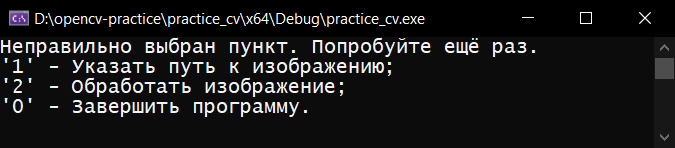
\includegraphics[width=0.9\textwidth]{menu_func.png}
 \caption{Запуск программы. Вызов функции menu.}\label{fig:par}
\end{figure}

\begin{figure}
 \centering
 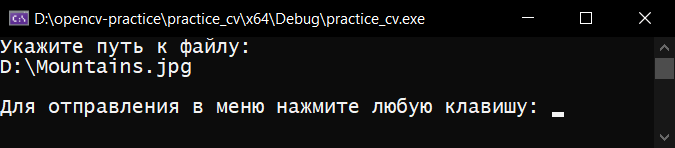
\includegraphics[width=0.9\textwidth]{image_get.png}
 \caption{Ввод пути изображения с клавиатуры.}\label{fig:par}
\end{figure}

\begin{figure}
 \centering
 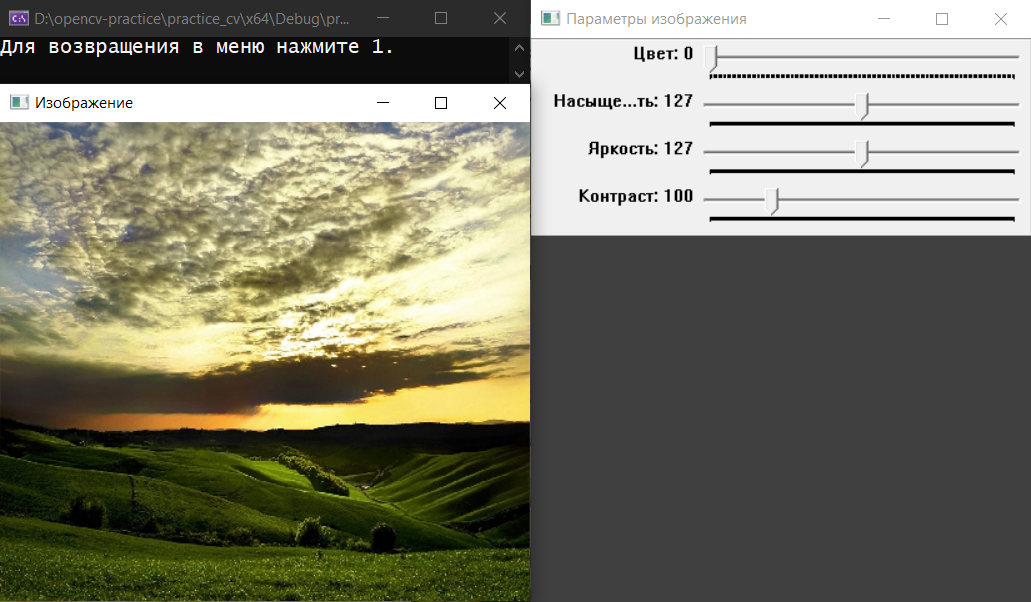
\includegraphics[width=1\textwidth]{image_edit.png}
 \caption{Выполнение функции обработки изображения. Создание окон.}\label{fig:par}
\end{figure}

\begin{figure}
 \centering
 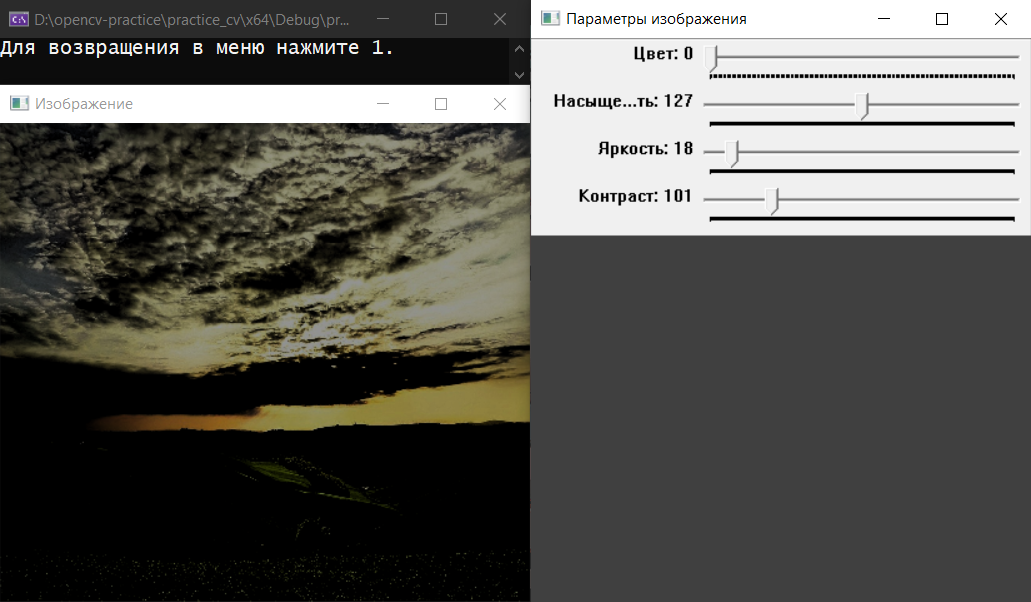
\includegraphics[width=1\textwidth]{image_edit_brightness.png}
 \caption{Изменение параметра яркости.}\label{fig:par}
\end{figure}

\begin{figure}
 \centering
 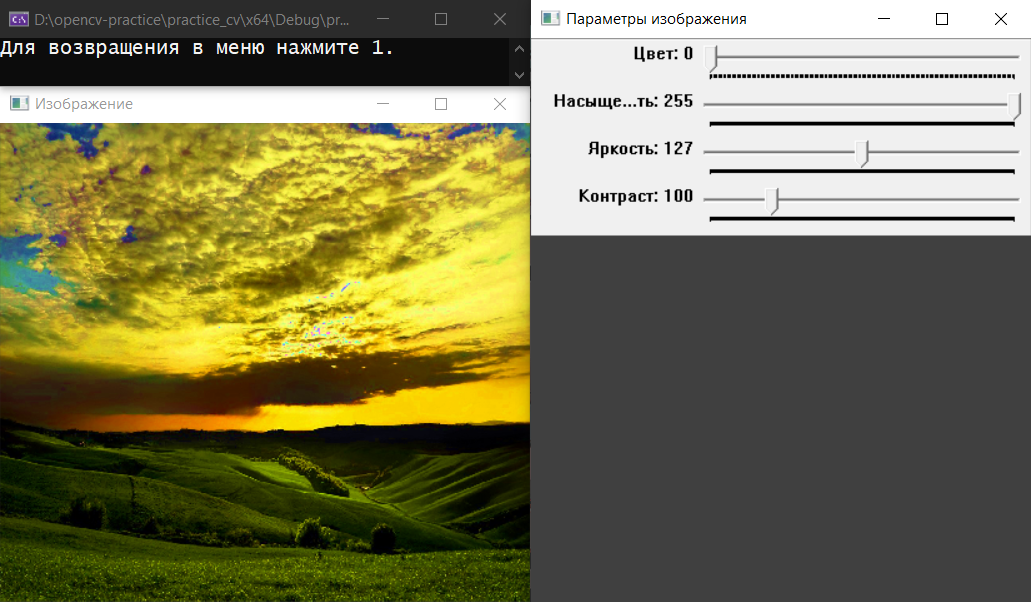
\includegraphics[width=1\textwidth]{image_edit_saturation.png}
 \caption{Изменение параметра насыщенности.}\label{fig:par}
\end{figure}

\begin{figure}
 \centering
 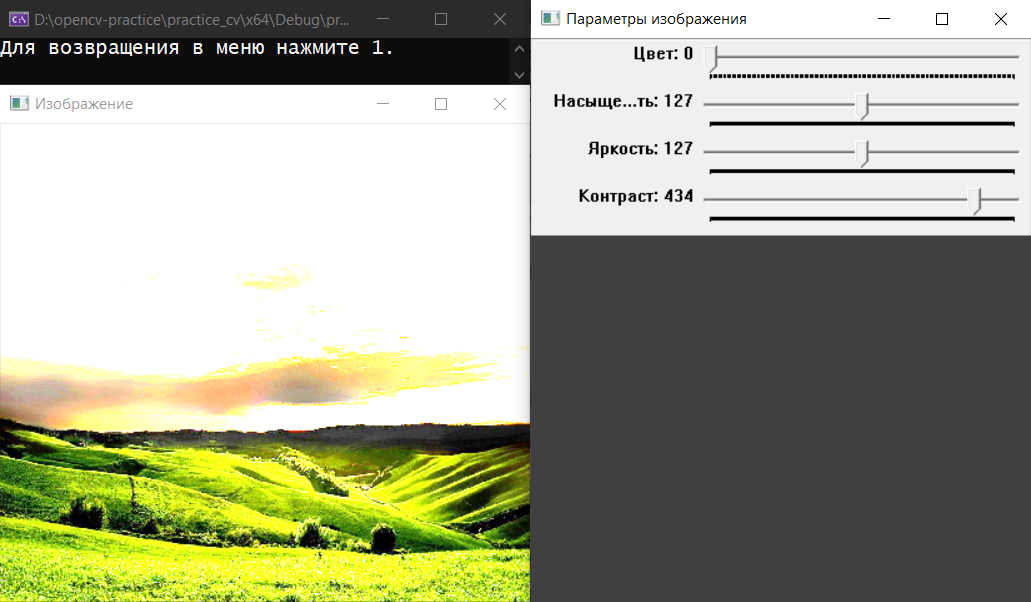
\includegraphics[width=1\textwidth]{image_edit_contrast.png}
 \caption{Изменение параметра контрастности.}\label{fig:par}
\end{figure}

\begin{figure}
 \centering
 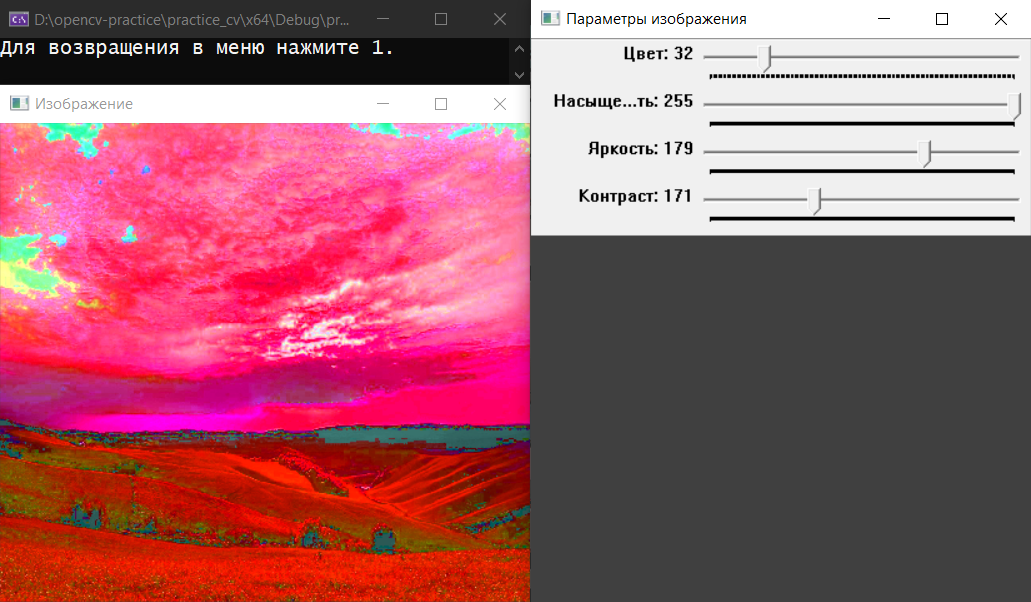
\includegraphics[width=1\textwidth]{image_edit_allparameters.png}
 \caption{Одновременное изменение всех параметров.}\label{fig:par}
\end{figure}

\end{document}